\documentclass[12pt, letterpaper]{article}
\date{\today}
\usepackage[margin=1in]{geometry}
\usepackage{amsmath}
\usepackage{hyperref}
\usepackage{cancel}
\usepackage{amssymb}
\usepackage{fancyhdr}
\usepackage{pgfplots}
\usepackage{booktabs}
\usepackage{pifont}
\usepackage{amsthm,latexsym,amsfonts,graphicx,epsfig,comment}
\pgfplotsset{compat=1.16}
\usepackage{xcolor}
\usepackage{tikz}
\usepackage{algpseudocode}
\usepackage{tabto}
\usetikzlibrary{shapes.geometric}
\usetikzlibrary{arrows.meta,arrows}
\newcommand{\Z}{\mathbb{Z}}
\newcommand{\N}{\mathbb{N}}
\newcommand{\R}{\mathbb{R}}
\newcommand{\Q}{\mathbb{Q}}
\newcommand{\C}{\mathbb{C}}
\newcommand{\F}{\mathbb{F}}

\newcommand{\Po}{\mathcal{P}}
\newcommand{\Pro}{\mathbb{P}}
\author{Alex Valentino}
\title{algos homework}
\pagestyle{fancy}
\renewcommand{\headrulewidth}{0pt}
\renewcommand{\footrulewidth}{0pt}
\fancyhf{}
\rhead{
	Homework 4\\
	CS 344	
}
\lhead{
	Alex Valentino\\
}
\begin{document}
\begin{enumerate}
	\item[3.25]
	\begin{enumerate}
		\item \begin{algorithmic}
		Input: $G = (V,E), v \in V$\\
		Output: cost\\
		\For{$u \in V$}
			$minCost = p_u$\\
			\For{$(v,u) \in $} 
			\State minCost = $\min{minCost, p_v}$
			\EndFor
		\EndFor
		\tab if not visited  
		\end{algorithmic}
		\item For a general digraph, one can first split up the digraph into it's strongly 
		connected components, just find the maximum cost per strongly connected node, then 
		run the algorithm as mentioned above on this newly formed graph.  This should take linear 
		time.  
	\end{enumerate}
	\item[4.1] 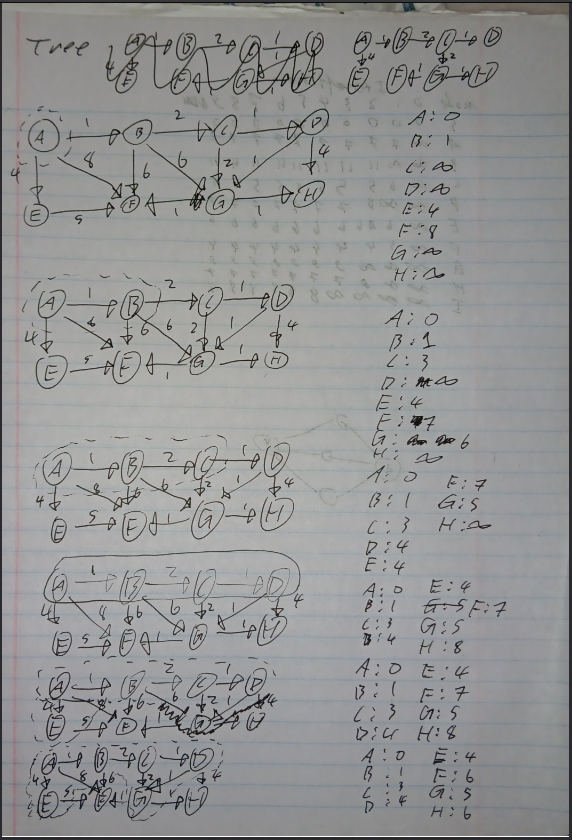
\includegraphics[scale=0.9]{algosHW541png.png}
	\item[4.2]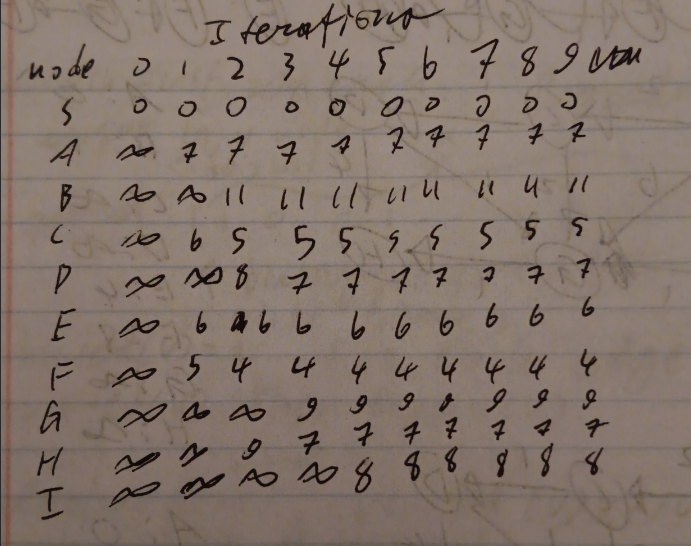
\includegraphics[scale=0.9]{algosHW542png.png}
	\item[4.5]
	\begin{algorithmic}
	Input Graph $G = (V,E)$, nodes $u,v \in V$\\
	Output minCons, the number of times $v$ is reached by a shortest
	connection
	\For{all $w \in V$}:
	\State seen$(w) = false$
	\EndFor\\
	
	dist$(u) =$ true\\
	seenv $=$ false\\
	minCons = 0\\
	$Q = [u]$\\
	\While{$Q$ is not empty}:
	\State w = eject $(Q)$
	 \For{all edges $(w,x) \in E$}:
	 \If{seen$(x) =$ false}
	 \If{$x = v$}
	 \State minCons$++$
	 \State seenv $=$ true
	 \Else
	  \State seen$(x)$ = true
	 \EndIf
	 \If{not seenv}
	 \State inject$(Q,w)$
	 \EndIf
	\EndIf
	\EndFor
	\EndWhile
	
	
	\end{algorithmic}
	Above is a modified version of BFS where we don't care 
	about distance.  Since BFS will have equal distance to every node
	when spreading out (unless it's a leaf and $v$ isn't encountered), all we care about is the first (minimal) 
	encounter with $v$, then from that point we stop putting 
	nodes on the stack and check if any other nodes in the same 
	distance will reach $v$, then we return the number of times 
	this occurs, giving us the number of equivalent minimal paths 
	from $u$ to $v$.  
	\item[chatGPT]
	\begin{algorithmic}
	Input Graph $G = (V,E)$, source $s \in V$\\
	Output whether or not the graph is bipartite or not\\
	\For{all $u \in V$}
		\State color$(u) = $ Null\\
	\EndFor\\
	color$(s) = $ true\\
	$Q = [s]$\\
	\While{$Q$ is not empty}
	\State $u = $ Eject$(Q)$
	\For{$(u,v) \in E$}
		\If{color$(v)$ = Null}
			\State color$(v)$ = not color$(u)$
			\State inject$(Q,v)$
		\ElsIf{color$(v)$ = color$(u)$}
			\State return false
		\EndIf
	\EndFor
	\EndWhile
	
	
	\end{algorithmic}
\end{enumerate}
\end{document}
